\documentclass[a4paper,12pt]{article}
\usepackage[utf8]{inputenc}
\usepackage[T1]{fontenc}
\usepackage[french]{babel}
\usepackage[right=2.5cm, left=2.5cm]{geometry}
\usepackage[ddmmyyyy]{datetime}
\usepackage[table]{xcolor}
\usepackage{lmodern,mathptmx,changepage,titlesec,hyperref,listings,lstautogobble,graphicx,array,longtable,multirow,lipsum,tikz,shorttoc,enumitem}
\usetikzlibrary{arrows,automata}
\usetikzlibrary{positioning}

\renewcommand{\rmdefault}{\sfdefault} %Utilisation de la police sans-serif ("Computer Modern Sans") pour la police roman
\renewcommand{\ttdefault}{pcr} 	%Utilisation d'une police "CourrierNew" pour la police monospaced (pour faire un listing manuel)
\linespread{1.15}				%Interligne

%Utilisation de liens colorés en bleu et soulignés
\hypersetup{colorlinks=true, urlcolor=blue, urlbordercolor=blue, linkcolor=black, linkbordercolor=white}
\makeatletter \Hy@AtBeginDocument{\def\@pdfborder{0 0 1} \def\@pdfborderstyle{/S/U/W 1}}\makeatother

\titlespacing*{\section} {0cm}{7ex plus 1ex minus .2ex}{1.5ex plus .2ex}
\titlespacing*{\subsection} {0cm}{4.5ex plus 1ex minus .2ex}{1.5ex plus .2ex}
\titleformat*{\section}{\huge\bfseries}
\titleformat*{\subsection}{\Large\bfseries}
\titleformat*{\subsubsection}{\normalsize\bfseries}

\definecolor{darkgreen}{rgb}{0,0.8,0}
\definecolor{mygray}{rgb}{0.93,0.93,0.93}
\definecolor{mymauve}{rgb}{0.58,0,0.82}
\lstset{	
	basicstyle=\small\ttfamily,
	backgroundcolor=\color{mygray},
	breaklines=true,
	breakatwhitespace=true,
	postbreak=\raisebox{0ex}[0ex][0ex]{\ensuremath{\color{red}\hookrightarrow\space}},
	tabsize=3,
	frame=none,
	rulecolor=\color{black},
	keywordstyle=\color{blue}\bfseries,
	stringstyle=\color{orange},
	showstringspaces=false,
	commentstyle=\footnotesize\color{darkgreen},
	keepspaces=true,
	extendedchars=true,
	numbers=left,
	numberstyle=\tiny\color{lightgray},
	stepnumber=1,
	escapeinside={(@}{@)},
	autogobble=true,
	literate=
		{á}{{\'a}}1 {é}{{\'e}}1 {í}{{}}1 {ó}{{\'o}}1 {ú}{{\'u}}1
		{Á}{{\'A}}1 {É}{{\'E}}1 {Í}{{\'I}}1 {Ó}{{\'O}}1 {Ú}{{\'U}}1
		{à}{{\`a}}1 {è}{{\`e}}1 {ì}{{\`i}}1 {ò}{{\`o}}1 {ù}{{\`u}}1
		{À}{{\`A}}1 {È}{{\'E}}1 {Ì}{{\`I}}1 {Ò}{{\`O}}1 {Ù}{{\`U}}1
		{ä}{{\"a}}1 {ë}{{\"e}}1 {ï}{{\"i}}1 {ö}{{\"o}}1 {ü}{{\"u}}1
		{Ä}{{\"A}}1 {Ë}{{\"E}}1 {Ï}{{\"I}}1 {Ö}{{\"O}}1 {Ü}{{\"U}}1
		{â}{{\^a}}1 {ê}{{\^e}}1 {î}{{\^i}}1 {ô}{{\^o}}1 {û}{{\^u}}1
		{Â}{{\^A}}1 {Ê}{{\^E}}1 {Î}{{\^I}}1 {Ô}{{\^O}}1 {Û}{{\^U}}1
		{œ}{{\oe}}1 {Œ}{{\OE}}1 {æ}{{\ae}}1 {Æ}{{\AE}}1 {ß}{{\ss}}1
		{ç}{{\c c}}1 {Ç}{{\c C}}1 {ø}{{\o}}1 {å}{{\r a}}1 {Å}{{\r A}}1
		{€}{{e}}1 {£}{{\pounds}}1 {«}{{\guillemotleft}}1
		{»}{{\guillemotright}}1 {ñ}{{\~n}}1 {Ñ}{{\~N}}1 {¿}{{?`}}1
}

%Redéfinition de la taille de \Huge pour le titre du document
\makeatletter\renewcommand\Huge{\@setfontsize\Huge{37pt}{40}}\makeatother
\date{\today}

\title{\vspace{\fill}\textbf{\Huge Spécifications}}
\author{
	Sonny Klotz - Jean-Didier Pailleux - Malek Zemni
	\vspace{2em}\\
	\textit{Interface de chargement, de contrôle}\\\textit{et d’analyse statistique des données}\\\textit{pour la constitution d’un graphe de flux}
	\vspace{2em}
}

\begin{document}
\pagenumbering{gobble}\clearpage
\maketitle\vspace{8em}
\begin{center}
\includegraphics[scale=0.7]{../Cahier/logo.png}\end{center}
\begin{flushright}Module \textit{Projet}\end{flushright}
\newpage
\tableofcontents
\newpage\clearpage\pagenumbering{arabic}

	\section*{Introduction}
		Ce document va décrire l'ensemble des exigences fonctionnelles que doit satisfaire notre produit final, c'est-à-dire les différentes fonctionnalités que notre application va fournir. Cette description va prendre en compte les caractéristiques des outils de développement choisis.
		\paragraph{}Notre outil, Python, est un langage de programmation hybride. On utilisera d'une part la programmation fonctionnelle pour les calculs, et d'autre part la programmation objet pour le développement des interfaces graphiques. Dans Python, le type de données n'est connu qu'à l'exécution (typage dynamique), par conséquent, ces types ne seront pas indiqués dans les signatures des fonctions et les structures des classes. Ils seront précisés dans des paragraphes explicatifs.
		\paragraph{}Pour les parties qui s'appuient sur une interaction avec l'utilisateur, notre démarche de description des fonctionnalités va essentiellement prendre en compte l'\textit{expérience utilisateur}\footnote{http://uxdesign.com/ux-defined}. Cette description sera donc axée sur la qualification du résultat et du ressenti de l'utilisateur lors de la manipulation de l'interface fournie (une illustration à l'aide de croquis), plutôt que sur les points techniques de l'application (fonctions et classes).
		\paragraph{}Les fonctionnalités de notre application seront présentées selon les modules de l'organigramme établi dans le cahier des charges. Ces modules eux-mêmes seront regroupés en packages. Ce document va donc décrire, pour chaque package de l'organigramme, les fonctionnalités de ses modules : d'abord ceux du package de chargement des données, puis ceux du package d'analyse descriptive des données et ensuite ceux du package de l'interface web. Les types Python utilisés seront décrits dans la dernière partie, le glossaire des types.
		
	\section{Package Chargement des données}
	Ce package est composé de 2 modules qui ont pour fonction de traiter le fichier de données fourni : une vérification de son format et une analyse de son contenu. On pourra aussi parler de API puisque ce package peut être éventuellement livré en sortie. 
		
		\subsection{Module Vérification format fichier}
			Ce module va vérifier le format du fichier de données fourni en entrée en 3 points. Il aura donc 3 fonctionnalités de vérification et une fonctionnalité globale d'ouverture du fichier.
			\begin{enumerate}
				\vspace{1em}\item Fonctionnalité de vérification de l'ouverture du fichier :
					\begin{lstlisting}
						verifOuverture(fichierCSV)
					\end{lstlisting}
					\underline{Paramètres :}
						\begin{description}[style=unboxed,leftmargin=0.2cm]
							\item\lstinline!fichierCSV! : \lstinline!TextIoWrapper! - représente le fichier CSV fourni.
						\end{description}
					\underline{Retour :} variable de type entier signalant un succès (0) ou une erreur (1).\\
					\underline{Description :} cette fonction prend en entrée le fichier CSV ouvert. Elle vérifie que le paramètre \lstinline!fichierCSV! contient bien des informations représentant un fichier quelconque, et renvoie l'entier 0 si c'est le cas, l'entier 1 sinon.
				\vspace{1em}\item Fonctionnalité de vérification de l'extension du fichier ouvert :
					\begin{lstlisting}
						verifExtenstion(fichierCSV)
					\end{lstlisting}
					\underline{Paramètres :}
						\begin{description}[style=unboxed,leftmargin=0.2cm]
							\item\lstinline!fichierCSV! : \lstinline!TextIoWrapper! - représente le fichier CSV fourni.
						\end{description}
					\underline{Retour :} variable de type entier signalant un succès (0) ou une erreur (2).\\
					\underline{Description :} cette fonction prend en entrée le fichier CSV ouvert. Elle vérifie que l'information décrivant l'extension du fichier dans le paramètre \lstinline!fichierCSV! correspond bien au format CSV, et renvoie l'entier 0 si c'est le cas, l'entier 2 sinon.
				\vspace{1em}\item Fonctionnalité de vérification de l'accessibilité en lecture du fichier :
					\begin{lstlisting}
						verifLecture(fichierCSV)
					\end{lstlisting}
					\underline{Paramètres :}
						\begin{description}[style=unboxed,leftmargin=0.2cm]
							\item\lstinline!fichierCSV! : \lstinline!TextIoWrapper! - représente le fichier CSV fourni.
						\end{description}
					\underline{Retour :} variable de type entier signalant un succès (0) ou une erreur (3).\\
					\underline{Description :} cette fonction prend en entrée le fichier CSV ouvert. Elle vérifie que le paramètre \lstinline!fichierCSV! représentant le fichier possède bien la propriété d'accès en lecture. Un test de lecture sera aussi effectué sur le fichier. La fonction renvoie l'entier 0 si l'accès en lecture est permis, l'entier 3 sinon.
				\vspace{1em}\item Fonctionnalité globale d'ouverture du fichier CSV :
					\begin{lstlisting}
						ouvrir(chemin)
					\end{lstlisting}
					\underline{Paramètres :}
						\begin{description}[style=unboxed,leftmargin=0.2cm]
							\item\lstinline!chemin! : \lstinline!str! - chaîne de caractères représentant le chemin relatif ou absolu du fichier CSV fourni.
						\end{description}
					\underline{Retour :} variable de type entier signalant un succès (0) ou une erreur (1, 2, ou 3).\\
					\underline{Description :} cette fonction prend en entrée le chemin du fichier CSV fourni. Elle ouvre ce fichier en lecture à l'aide de la fonction \lstinline!open(chemin,"r")! et le stocke dans une variable de type \lstinline!TextIoWrapper!. Elle applique ensuite dans l'ordre les trois fonctions de vérifications du module et renvoie le code de la fonction qui fait échouer l'ouverture (l'entier 1, 2 ou 3), ou bien un code signalant le succès de l'ouverture (l'entier 0).
			\end{enumerate}
		
		
		\subsection{Module Analyse contenu fichier}
			Ce module va analyser le contenu du fichier fourni en lisant une à une les données de ce fichier et en repérant les données erronées. Il aura donc 2 fonctionnalités :
			\begin{enumerate}
				\vspace{1em}\item Fonctionnalité de lecture du contenu du fichier CSV :
					\begin{lstlisting}
						lecture(fichierCSV)
					\end{lstlisting}
					\underline{Paramètres :}
						\begin{description}[style=unboxed,leftmargin=0.2cm]
							\item\lstinline!fichierCSV! : \lstinline!TextIoWrapper! - représente le fichier CSV fourni.
						\end{description}
					\underline{Retour :} une variable de type \lstinline!list! : une liste dont chaque élément est un dictionnaire contenant les données d'une ligne du fichier CSV.\\
					\underline{Description :} cette fonction prend en entrée le fichier CSV ouvert. Elle crée une liste pour y sauvegarder le contenu de ce fichier, ligne par ligne. Elle lit les caractères du fichier en entier à l'aide de la fonction \lstinline!read()!. Ensuite, pour chaque ligne du fichier, elle applique la fonction \lstinline!split(',')! pour séparer les caractères de cette ligne selon la virgule et les stocker dans un dictionnaire qui sera finalement stocké dans la liste englobante. L'utilisation d'un dictionnaire permet d'indexer les données de la ligne par le nom de la colonne : 
					\begin{lstlisting}
						[ 	
							{"nomColonne1" : donnée1Ligne1, "nomColonne2" donnée2Ligne1},
							{"nomColonne1" : donnée1Ligne2, "nomColonne2" donnée2Ligne2} 
						] 
					\end{lstlisting}
					Ces noms de colonnes proviennent du fichier CSV.
					
				\vspace{1em}\item Fonctionnalité de description du type et des erreurs des colonnes du fichier CSV :
					\begin{lstlisting}
						descriptionColonnes(lignesCSV)
					\end{lstlisting}
					\underline{Paramètres :}
						\begin{description}[style=unboxed,leftmargin=0.2cm]
							\item\lstinline!lignesCSV! : \lstinline!list! - liste représentant les données du fichier CSV ligne par ligne.
						\end{description}
					\underline{Retour :} une variable de type \lstinline!dict! : un dictionnaire de 2 dictionnaires indexés par \lstinline!"types"! et \lstinline!"erreurs"!.\\
					\underline{Description :} cette fonction prend en entrée le fichier CSV préalablement lu et stocké dans la liste \lstinline!lignesCSV!. Elle crée un dictionnaire de 2 éléments de type dictionnaire également, pour y renseigner le type et les erreurs de chaque colonne de ce fichier.\\
					Elle remplit d'abord le champ \lstinline!types! du dictionnaire par les types attendus. Ensuite, elle lit la liste \lstinline!lignesCSV! colonne par colonne. Pour chaque donnée d'une colonne, elle compare son type au type attendu et, en cas d'erreur, renseigne le numéro de cette ligne dans une liste dans le champ \lstinline!erreurs! du dictionnaire.
					\begin{lstlisting}
						{ 	
							"types" : {"nomColonne1" : typeColonne1, "nomColonne2" typeColonne2},
							"erreurs" : 
							{
								"nomColonne1" : [liste des numéros de lignes des données erronées de la colonne 1], 
								"nomColonne2" : [liste des numéros de lignes des données erronées de la colonne 2]
							} 
						} 
					\end{lstlisting}
			\end{enumerate}
	
	\section{Package Analyse descriptive des données}
	Ce package est composé de trois modules d'analyse descriptive de données. Ces informations pourront être utilisées pour le filtrage des valeurs dans l'échantillon de la fenêtre rôle et choix colonne, mais aussi servir pour les compte-rendu statistiques des colonnes.
	Ce package va être livré au client pour une intégration externe. On pourra donc parler de API.
	
		\subsection{Module Analyse de données qualitatives}
			Ce module va effectuer les calculs d'effectifs, d'effectifs cumulés, de fréquences et de fréquences cumulés. Il s'occupera également de fournir les informations nécessaire pour la construction d'un diagramme de secteur et d'un histogramme. Il aura donc 6 fonctionnalités :
	
			\begin{enumerate}
				\vspace{1em}\item Fonctionnalité de calcul de l'effectif :
					\begin{lstlisting}
						calculEffectif(donneeQualitative)
					\end{lstlisting}
					\underline{Paramètres :} 
					\begin{description}[style=unboxed,leftmargin=0.2cm]
						\item\lstinline!donneeQualitative! : \lstinline!list! - structure contenant les données de type qualitatif de la colonne.
					\end{description}
					\underline{Retour :} variable de type  \lstinline!list! : représente la sortie du calcul des effectifs de chaque valeur de la colonne.\\
					\underline{Description :} cette fonction prendra en paramètre une liste qui contiendra les données de type qualitatif pour le calcul. Elle calculera les effectifs pour chaque valeur et effectuera un tris pour ordonner ces valeurs.
					
				\vspace{1em}\item Fonctionnalité de calculer de l'effectif cumulé :
					\begin{lstlisting}
						calculEffectifCumule(listeEffectif)
					\end{lstlisting}
					\underline{Paramètres :} 
					\begin{description}[style=unboxed,leftmargin=0.2cm]
						\item\lstinline!listeEffectif! : \lstinline!list! - correspond au résultat de la fonction \lstinline!calculEffectif!.
					\end{description}
					\underline{Retour :} \lstinline!listeEffectif! : \lstinline!list! : copie de \lstinline!listeEffectif! mais dont les effectifs seront remplacé par les effectifs cumulés. \\
					\underline{Description :} cette fonction prend en entrée les résultats de la fonction \lstinline!calculEffectif! préalablement stocké dans une liste. Elle va copier dans une nouvelle liste celle rentrée en paramètre, et remplacera les effectifs par les effectifs cumulés. La fonction retournera cette nouvelle liste.
					
				\vspace{1em}\item Fonctionnalité pour calculer la fréquence :
					\begin{lstlisting}
						calculFrequence(donneeQualitative)
					\end{lstlisting}
					\underline{Paramètres :} 
					\begin{description}[style=unboxed,leftmargin=0.2cm]
						\item\lstinline!donneeQualitative! : \lstinline!list! - structure contenant les données de type qualitatif de la colonne.
					\end{description}
					\underline{Retour :} variable de type  \lstinline!list! - correspondant à la sortie du calcul des fréquences de chaque valeur de la colonne.\\
					\underline{Description :} cette fonction prendra en paramètre une liste qui contiendra les données de type qualitatif pour le calcul. Elle calculera les fréquences pour chaque valeur et effectuera un tris pour ordonner ces valeurs.
					
				\vspace{1em}\item Fonctionnalité pour calculer la fréquence cumulé :
					\begin{lstlisting}
						calculFrequenceCumule(listeFrequence)
					\end{lstlisting}
					\underline{Paramètres :} 
					\begin{description}[style=unboxed,leftmargin=0.2cm]
						\item\lstinline!listeFrequence! : \lstinline!list! - correspond au résultat de la fonction \lstinline!calculFrequence!.
					\end{description}
					\underline{Retour :} variable de type  \lstinline!list! - copie de \lstinline!listFréquence! mais dont les fréquences seront remplacé par les fréquences cumulés. \\
					\underline{Description :} cette fonction prend en entrée les résultats de la fonction \lstinline!calculFrequence! préalablement stocké dans une liste. Elle va copier dans une nouvelle liste celle rentrée en paramètre, et remplacera les fréquences par les fréquences cumulés. La fonction retournera cette nouvelle liste.
					
				\vspace{1em}\item Fonctionnalité pour les données du diagramme en secteur :
					\begin{lstlisting}
						infoSecteur(frequence)
					\end{lstlisting}
					\underline{Paramètres :} 
					\begin{description}[style=unboxed,leftmargin=0.2cm]
						\item \lstinline!frequence! :  \lstinline!list! - correspondant à la sortie du calcul des fréquences.
					\end{description}
					\underline{Retour :} fichier au format  \lstinline!.json! - contenant les informations nécessaire pour la construction d'un diagramme de secteur.\\
					\underline{Description :} cette fonction prend en entrée le résultat du calcul des fréquences préalablement stocké dans une liste \lstinline!frequence!. Elle va créer un fichier  \lstinline!.json!  pour y stocker les données pour construire le diagramme de secteur. Pour chaque couple (fréquence-valeur) elle va associer un angle compris entre 0\degre et 360\degre tel que la somme de tout les angles soit égale à 360\degre.
					
				\vspace{1em}\item Fonctionnalité pour les données de l'histogramme :
					\begin{lstlisting}
						infoHistogramme(effectif)
					\end{lstlisting}
					\underline{Paramètres :} 
					\begin{description}[style=unboxed,leftmargin=0.2cm]
						\item \lstinline!effectif! : \lstinline!list! - correspondant à la sortie du calcul des effectifs.
					\end{description}
					\underline{Retour :} fichier au format  \lstinline!.json! - contenant les informations nécessaire pour la construction d'un histogramme.\\
					\underline{Description :} cette fonction prend en entrée le résultat du calcul des effectifs préalablement stocké dans une liste \lstinline!effectif!. Elle va créer un fichier  \lstinline!.json! pour y stocker les données pour construire l'histogramme.
			\end{enumerate}
		
		\subsection{Module Analyse de données quantitatives discrètes}
			
		\subsection{Module Analyse de données quantitatives continues}
		
		
	\section{Package Interface web}
		Ce package est composé de 3 modules de fenêtre graphique web qui assurent l'interaction avec l'utilisateur, et d'un module de gestion des flux qui s'occupe du lancement de l'application et de la transition des informations entre ses différents packages.
		
		\subsection{Module Gestion des flux}
		Ce module va lancer l'application et sera au centre du programme. Il s'occupera de gérer les branchements pour l'exécution, de communiquer les informations entre les différents modules et arrêtera le programme en cas d'erreur. Il aura \colorbox{yellow}{??} fonctionnalités ainsi que le \lstinline!main! de l'application:
		
		\begin{enumerate} 
				\vspace{1em}\item La fonction main.
					\begin{lstlisting}
						main()
					\end{lstlisting}
					\underline{Paramètres :}
						\begin{description}[style=unboxed,leftmargin=0.2cm]
							\item Ne prend aucun paramètre.
						\end{description}
					\underline{Retour :} Ne retourne rien.\\
					\underline{Description :} la fonction \lstinline!main()! ne prend aucun paramètre en entrée et ne retourne rien en sortie. Elle s'occupe de lancer l'application en faisant appel à la première fenêtre choix fichier, et de faire tourner l'application. Elle s'occupe également de gérer les erreurs et donc de l'arrêt du programme. 
					
				\vspace{1em}\item Fonctionnalité pour générer la fenêtre choix fichier.
					\begin{lstlisting}
						choix_fichier()
					\end{lstlisting}
					\underline{Paramètres :}
						\begin{description}[style=unboxed,leftmargin=0.2cm]
							\item Ne prend aucun paramètre.
						\end{description}
					\underline{Retour :} \lstinline!render_template()! : fonction qui renvoie le contenu de la page web mis en paramètre qui va être envoyée au client. \\
					\underline{Description :} cette fonction correspond à la requête HTTP (c'est à dire le chemin de la page demandée) envoyée par le client et reçue par le serveur qui sera soit un GET soit un POST. Pour cela il faudra indiquer avant de déclarer la fonction la ligne suivante : \lstinline!@app.route('/choix_fichier/', methods=['GET', 'POST'])!. Elle retournera le contenu de la page web mis en paramètre de la fonction \lstinline!render_template()! associé au code \lstinline!HTML! de la fenêtre choix fichier. Des variables en tant qu'arguments optionnels peuvent-être utilisé dans le cas où l'on souhaiterait afficher des valeurs.
					
				\vspace{1em}\item Fonctionnalité pour générer la fenêtre rôle et choix colonne.
					\begin{lstlisting}
						role_choix_colonne()
					\end{lstlisting}
					\underline{Paramètres :}
						\begin{description}[style=unboxed,leftmargin=0.2cm]
							\item Ne prend aucun paramètre.
						\end{description}
					\underline{Retour :} \lstinline!render_template()! : fonction qui renvoie le contenu de la page web mis en paramètre qui va être envoyée au client. \\
					\underline{Description :} cette fonction correspond à la requête HTTP (c'est à dire le chemin de la page demandée) envoyée par le client et reçue par le serveur qui sera soit un GET soit un POST. Pour cela il faudra indiquer avant de déclarer la fonction la ligne suivante : \lstinline!@app.route('/role_choix_colonne/', methods=['GET', 'POST'])!. Elle retournera le contenu de la page web mis en paramètre de la fonction \lstinline!render_template()! associé au code \lstinline!HTML! de la fenêtre rôle et choix colonne. Des variables en tant qu'arguments optionnels peuvent-être utilisé dans le cas où l'on souhaiterait afficher des valeurs.
					
				\vspace{1em}\item Fonctionnalité pour générer la fenêtre résultats ADD.
					\begin{lstlisting}
						resultat_ADD()
					\end{lstlisting}
					\underline{Paramètres :}
						\begin{description}[style=unboxed,leftmargin=0.2cm]
							\item Ne prend aucun paramètre.
						\end{description}
					\underline{Retour :} \lstinline!render_template()! : fonction qui renvoie le contenu de la page web mis en paramètre qui va être envoyée au client. \\
					\underline{Description :} cette fonction correspond à la requête HTTP (c'est à dire le chemin de la page demandée) envoyée par le client et reçue par le serveur qui sera soit un GET soit un POST. Pour cela il faudra indiquer avant de déclarer la fonction la ligne suivante : \lstinline!@app.route('/resultat_ADD/', methods=['GET', 'POST'])!. Elle retournera le contenu de la page web mis en paramètre de la fonction \lstinline!render_template()! associé au code \lstinline!HTML! de la fenêtre résultat ADD. Des variables en tant qu'arguments optionnels peuvent-être utilisé dans le cas où l'on souhaiterait afficher des valeurs.
					
				\vspace{1em}\item Fonctionnalité pour la validation du choix colonne. \colorbox{yellow}{En attente de Malek}
					\begin{lstlisting}
						validChoixColonne(signal)
					\end{lstlisting}
					\underline{Paramètres :}
						\begin{description}[style=unboxed,leftmargin=0.2cm]
							\item \lstinline!signal! : 
						\end{description}
					\underline{Retour :} \\
					\underline{Description :} 
					
				\vspace{1em}\item Fonctionnalité pour la demande d'exportation. \colorbox{yellow}{En attente de Sonny}
					\begin{lstlisting}
						demandeExport(signal)
					\end{lstlisting}
					\underline{Paramètres :}
						\begin{description}[style=unboxed,leftmargin=0.2cm]
							\item \lstinline!signal! : 
						\end{description}
					\underline{Retour :} \\
					\underline{Description :} 
										
					\end{enumerate}
		
		\subsection{Module Fenêtre choix fichier}
		Ce module est une fenêtre graphique web qui va permettre à l'utilisateur de charger un fichier CSV. Il aura 3 fonctionnalités :

			\begin{enumerate}
				\vspace{1em}\item Fonctionnalité pour ouvrir le fichier avec le Système de Gestion de fichier :
					\begin{lstlisting}
						FileWithSGF()
					\end{lstlisting}
					\underline{Paramètres :} 
					\begin{description}[style=unboxed,leftmargin=0.2cm]
						\item Ne demande aucun paramètre en entrée.
					\end{description}
					\underline{Retour :} variable de type \lstinline!str! - chaîne de caractères représentant le chemin relatif ou absolu du fichier CSV fourni.\\
					\underline{Description :} cette fonction ne prend pas de paramètre en entrée. Elle permet de récupérer  l'emplacement du fichier CSV avec la technique du Drag\&Drop. Elle renvoie donc une chaîne de caractères correspondant à ce chemin.
					
				\vspace{1em}\item Fonctionnalité pour ouvrir le fichier avec la technique du Drag\&Drop.
					\begin{lstlisting}
						FileWithDragDrop()
					\end{lstlisting}
					\underline{Paramètres :} 
					\begin{description}[style=unboxed,leftmargin=0.2cm]
						\item Ne demande aucun paramètre en entrée.
					\end{description}
					\underline{Retour :} variable de type \lstinline!str! - chaîne de caractères représentant le chemin relatif ou absolu du fichier CSV fourni.\\
					\underline{Description :} cette fonction ne prend pas de paramètre en entrée. Elle permet de récupérer l'emplacement du fichier CSV en parcourant le système de gestion de fichiers. Elle renvoie donc une chaîne de caractères correspondant à ce chemin.

				\vspace{1em}\item Aspect visuel.
				
				\paragraph{}Le croquis ci-dessous représente la fenêtre avant d'avoir choisi un fichier. Le chemin relatif ou absolu sera être renseigné soit en déplaçant dans la zone en pointillé ce dernier, soit en cliquant sur le symbole "+" pour parcourir le système de gestion de fichiers:
					\begin{center}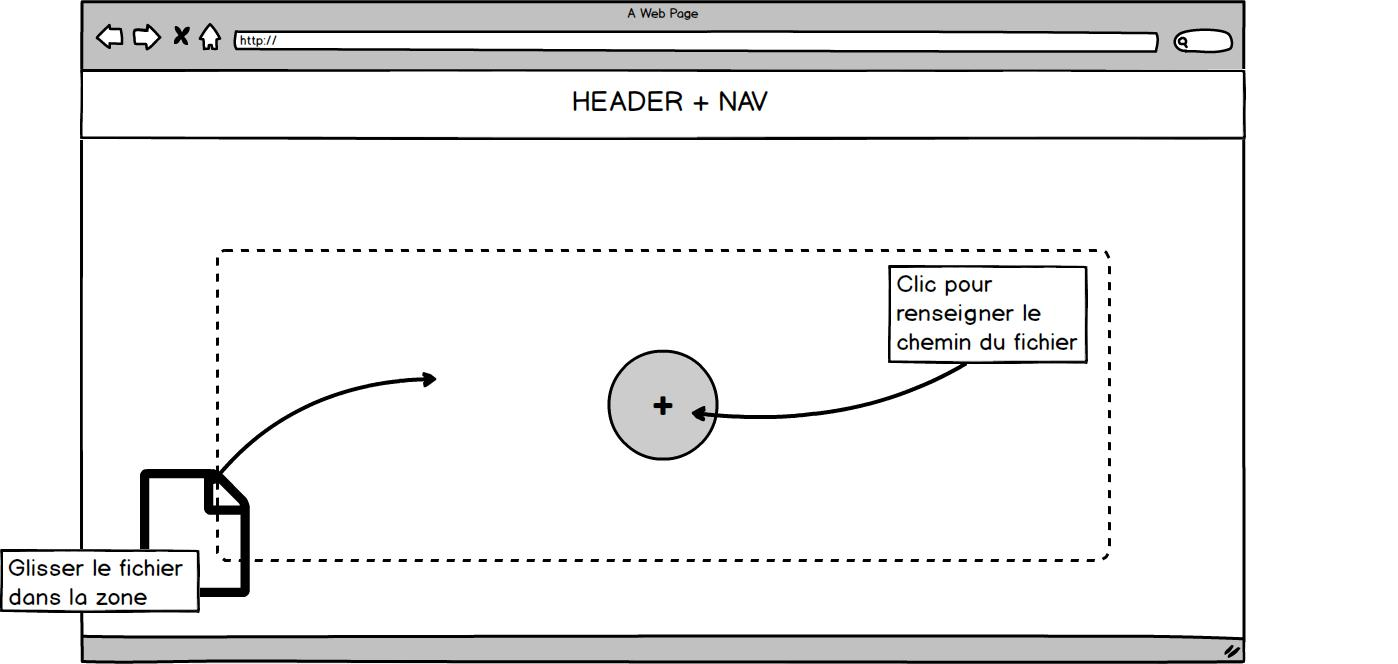
\includegraphics[scale=0.57]{Fenetre_choix_fichier1.jpg}\end{center} 
					
				\paragraph{}La fenêtre prendra ensuite l'apparence du croquis suivant lorsque l'utilisateur aura choisi un fichier. Son chemin sera affiché à l'écran. A côté de celui-ci sera affiché un indicateur pour la validité du fichier, et un bouton pour supprimé le choix. Dans le dernier cas, la fenêtre reprendra sa première apparence. Puis un bouton sera afficher pour valider le choix:
					
					\begin{center}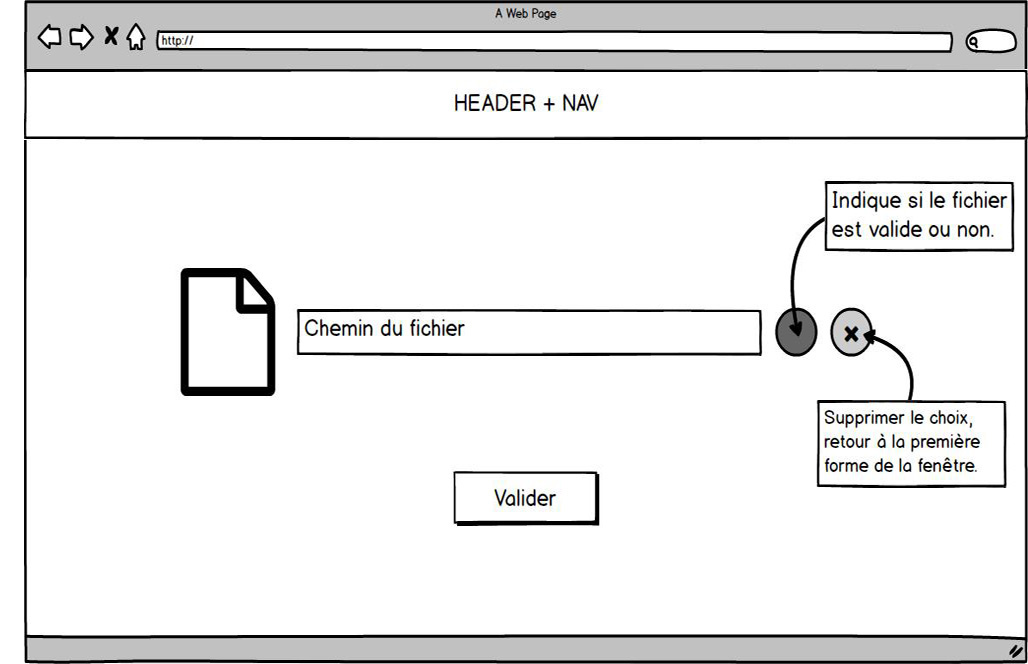
\includegraphics[scale=0.5]{Fenetre_choix_fichier2.jpg}\end{center}
				\paragraph{}Les deux fenêtres abordent une apparence simple et épuré. L'effet cherché est que lorsque l'utilisateur regardera la fenêtre, il devra tout de suite comprendre comment elle fonctionnera.

			\end{enumerate}
			
		\subsection{Module Fenêtre rôle et choix colonne}
			Ce module est une fenêtre graphique web qui permet d'une part d'afficher un échantillon filtré des données du fichier et ses informations relatives, et d'autre part, de choisir une colonne de cet échantillon pour l'analyser. Ce module aura 3 fonctionnalités qui peuvent être illustrées par ce croquis :
			\begin{center}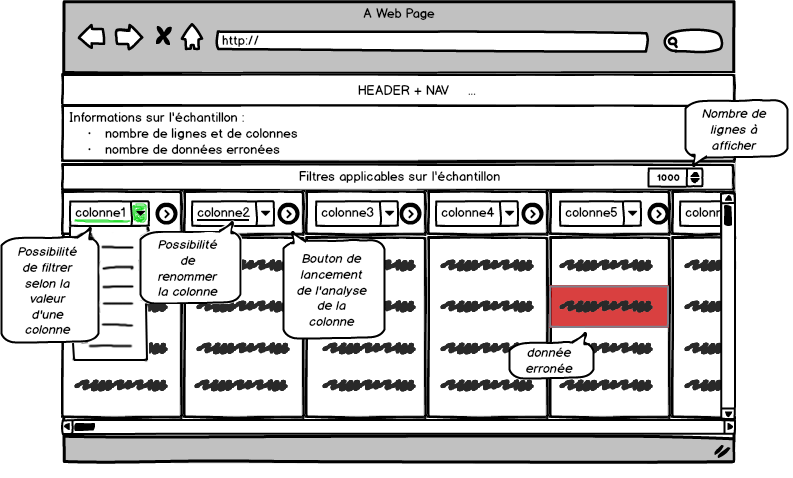
\includegraphics[scale=0.5]{fenetreEchantillons.png}\end{center}
			\begin{enumerate}
				\vspace{1em}\item Fonctionnalité d'affichage de l'échantillon :
				\vspace{1em}\item Fonctionnalité de filtrage de l'échantillon :
				\vspace{1em}\item Fonctionnalité de choix de colonne à analyser :
			\end{enumerate}
			
			
		\subsection{Module Fenêtre résultats ADD}
			Ce module décrit la fenêtre dans laquelle l'utilisateur de l'applet pourra consulter les résultats d'analyse des colonnes du fichier importé.
			\begin{enumerate}
				\item \underline{Aspect visuel :}\\
					\begin{center}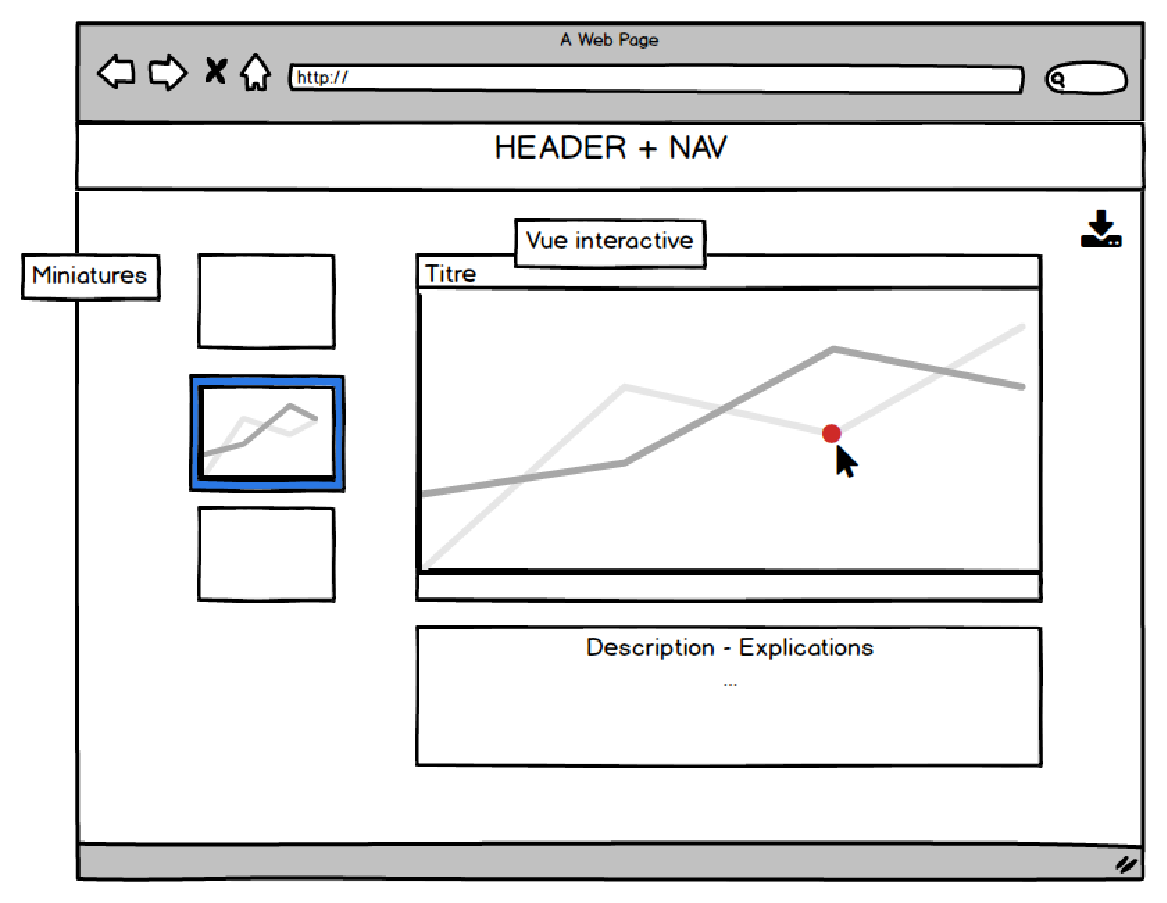
\includegraphics[scale=0.8]{FenetreADD.pdf}\end{center}
					Les résultats doivent se présenter de manière simple et sans surcharge. Les utilisateurs de ce produit doivent pouvoir prendre en main et comprendre les données sans pour autant être formés. C'est pour cela que l'information se limite à un bouton, des reprèsentations graphiques, et des explications générées à laide des calculs d'analyse descriptive.
				\item \underline{Intéractions avec l'utilisateur :}\\
					\begin{itemize}
						\item Miniatures : Un clic sur une miniature permet de la faire basculer en vue précise.
						\item Vue précise : Un affichage interactif des valeurs rend la consultation plus intuitive et la charge de la vue plus légère. (une valeur non-demandée n'est pas affichée)
						\item Sauvegarde des résultats : Une simple icône de téléchargement permettra de lancer la sauvegarde des résultats en local.
					\end{itemize}
				\item \underline{Vues précises :}\\
					Ci-dessous, une liste des représentations graphiques disponibles, ainsi que le type d'analyse qui permet de les afficher :
					\begin{itemize}
						\item Histogramme : ADD\footnote{ADD : analyse descriptive de données} qualitatives
						\item Diagramme en secteur : ADD qualitatives
						\item Série temporelle : ADD quantitatives
						\item Distribution des valeurs : ADD quantitatives
						\item Distribution cumulative des valeurs : ADD quantitatives
						\item Diagramme à moustaches : ADD quantitatives
			\end{enumerate}
	
	\section{Glossaire des types}
		Dans ce glossaire, on va préciser la définition des types des données qu'on a utilisé dans la description des fonctionnalités.
		\begin{itemize}
			\item \lstinline!TextIoWrapper! : classe représentant les flux de texte bufferisés (entrées/sorties de texte avec une sauvegarde dans une mémoire tampon). Elle permet donc de représenter les fichiers de texte brut en particulier. Elle définit des méthodes de manipulation de ces flux.
			\item \lstinline!str! : classe représentant des séquences de caractères (donc des chaînes de caractères) en Python. Elle définit des méthodes de manipulation de ces chaînes.
			\item \lstinline!list! : classe représentant des séquences de variables de type quelconque indexés par des entier. Elle définit des méthodes de manipulation de ces séquences.\\
				L'utilisation de ce type de données pour la manipulation des colonnes du fchier \lstinline!.csv! est préconisée car, tout d'abord, le type et les fonctions de manipulations sont disponibles directement avec Python, ensuite, ces listes sont implémentées sous forme de tableau ce qui garantie l'accès rapide à chacun de ses éléments, et enfin, leur taille maximale est définie par l'entier \lstinline!sys.maxsize! qui dépend des machines mais dépasse largement le million sur des PC bureautiques standards. Le million correspond à une borne maximale du nombre de lignes du fichier \lstinline!.csv! importé, la manipulation des listes peut donc se faire sans risque de crash mémoire.
			\item \lstinline!dict! : classe représentant des séquences de couple clés, variables (indexés par cette clé). Elle définit des méthodes de manipulation de ces séquences.		
			\item \lstinline!tuple! : classe représentant des listes immuables (non modifiables).
			\item \lstinline!.json! : (JavaScript Object Notation) format de données textuelles basé sur la notation des objets JavaScript. C'est un moyen simple d'accéder à des données car un flux JSON est une sérialisation (une traduction) d'un objet JavaScript.
 		\end{itemize}
	
	\section*{Conclusion}
		Bilan : rappel ce qu'on a fait et ce que ça a apporté\\
		Ouvertures :\\
			- Mise en place des tests d'acceptations (comment on va mesurer, il faut définir une mesure et après la calculer)\\
			-->fct : type retour 1 unite, chaque parametre 1 unite\\
			-->classe : chaque attribut 1 unite, methode comme fct\\
			-->représentation grpahique :  ??? depend de c3js\\
			-->fenêtre : ??? dépend des croquis, de flask\\
			-->fenêtre et representation graphq, specs pas forcément  représentatives => pas de mesure ??  (voire limites)\\
			-->mesure = nombre d'unites obtenues / nombre d'unites possibles
			-->relever la position des écarts techniques en même temps
			- Difficultés\\
			- Limites des spécifications dans notre cas : nécessité de tester une 1ere version de l'appli pour bien définir l'expérience utilisateur\\
		Dernière phrase positive :\\
			- Découverte nouveaux outils, nouvelle démarche pour le dev : devops, ux design, balsamiq, les app web (javascript c'est assez bien en vrai)
		
\end{document}
